%%%%%%%%%%%%%%%%%%%%%%%%%%%%%%%%%%%%%%%%%%%%%%%%%%%%%%%%%%%%%%%%%%%%%%%%%%%
%% This file is part of the book
%%
%% Algorithmic Graph Theory
%% http://code.google.com/p/graph-theory-algorithms-book/
%%
%% Copyright (C) 2009--2011 Minh Van Nguyen <nguyenminh2@gmail.com>
%%
%% See the file COPYING for copying conditions.
%%%%%%%%%%%%%%%%%%%%%%%%%%%%%%%%%%%%%%%%%%%%%%%%%%%%%%%%%%%%%%%%%%%%%%%%%%%

%% See the file gnp.c for a C program that generates the experimental
%% and expected results used in deriving the results below.

\documentclass{article}

\usepackage{pgfplots}
\usetikzlibrary{external}
\tikzexternalize{Gnp-simulation}

\begin{document}

\begin{figure}
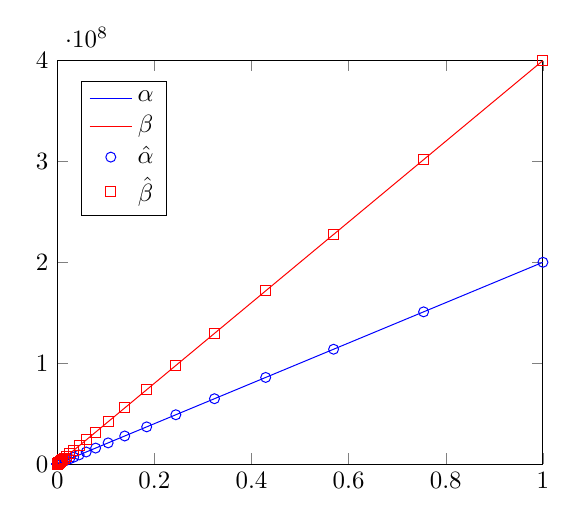
\begin{tikzpicture}
[every mark/.append style={scale=1},%
 scale=0.9]
\begin{axis}[%
  enlargelimits=false,%
  legend style={at={(0.225,0.95)}}%
]
%% xn(n - 1) / 2
\addplot[color=blue] expression[domain=0:1] {199990000*x};
%% xn(n - 1)
\addplot[color=red] expression[domain=0:1] {399980000*x};
\addplot+[only marks,color=blue,mark=o] coordinates
{
  (1.00000000000000e-6, 199.434000000000)
  (1.32571133853476e-6, 265.780000000000)
  (1.75751055311963e-6, 352.760000000000)
  (2.32995166786519e-6, 464.084000000000)
  (3.08884334432687e-6, 616.934000000000)
  (4.09491464453176e-6, 820.308000000000)
  (5.42867477458780e-6, 1085.47600000000)
  (7.19685570188869e-6, 1439.25400000000)
  (9.54095320579239e-6, 1903.19800000000)
  (0.0000126485498453486, 2530.86800000000)
  (0.0000167683259460007, 3354.24400000000)
  (0.0000222299598348597, 4440.89600000000)
  (0.0000294705098082459, 5891.58200000000)
  (0.0000390693890051915, 7810.72800000000)
  (0.0000517947319938078, 10356.6260000000)
  (0.0000686648634805601, 13734.8340000000)
  (0.0000910297880751201, 18204.2820000000)
  (0.000120679222195603, 24142.3820000000)
  (0.000159985813190267, 31978.7660000000)
  (0.000212095006551041, 42416.2280000000)
  (0.000281176755031320, 56232.2820000000)
  (0.000372759212277432, 74568.2100000000)
  (0.000494171114259478, 98818.1660000000)
  (0.000655128249350147, 131058.564000000)
  (0.000868510948357918, 173692.452000000)
  (0.00115139481187967, 230289.120000000)
  (0.00152641715723898, 305262.886000000)
  (0.00202358853268571, 404691.088000000)
  (0.00268269426231037, 536531.076000000)
  (0.00355647820136701, 711266.308000000)
  (0.00471486347680396, 942929.208000000)
  (0.00625054797084244, 1.25005086200000e6)
  (0.00828642231700127, 1.65720860600000e6)
  (0.0109854040215361, 2.19696968200000e6)
  (0.0145634746697357, 2.91261120800000e6)
  (0.0193069634981325, 3.86130230600000e6)
  (0.0255954604221510, 5.11885376200000e6)
  (0.0339321920966633, 6.78596425200000e6)
  (0.0449842918038862, 8.99627065600000e6)
  (0.0596361857003683, 1.19264806480000e7)
  (0.0790603675699428, 1.58113832900000e7)
  (0.104811225716199, 2.09610549820000e7)
  (0.138949430337692, 2.77885028420000e7)
  (0.184206835281624, 3.68395862100000e7)
  (0.244205090168454, 4.88387172280000e7)
  (0.323745456964223, 6.47460697980000e7)
  (0.429193023096588, 8.58344541200000e7)
  (0.568986057139159, 1.13791283798000e8)
  (0.754311267417571, 1.50854683924000e8)
  (0.999999000000001, 1.99989800522000e8)
};
%%
\addplot+[only marks,color=red,mark=square] coordinates
{
  (1.00000000000000e-6, 398.868000000000)
  (1.32571133853476e-6, 531.560000000000)
  (1.75751055311963e-6, 705.520000000000)
  (2.32995166786519e-6, 928.168000000000)
  (3.08884334432687e-6, 1233.86800000000)
  (4.09491464453176e-6, 1640.61600000000)
  (5.42867477458780e-6, 2170.95200000000)
  (7.19685570188869e-6, 2878.50800000000)
  (9.54095320579239e-6, 3806.39600000000)
  (0.0000126485498453486, 5061.73600000000)
  (0.0000167683259460007, 6708.48800000000)
  (0.0000222299598348597, 8881.79200000000)
  (0.0000294705098082459, 11783.1640000000)
  (0.0000390693890051915, 15621.4560000000)
  (0.0000517947319938078, 20713.2520000000)
  (0.0000686648634805601, 27469.6680000000)
  (0.0000910297880751201, 36408.5640000000)
  (0.000120679222195603, 48284.7640000000)
  (0.000159985813190267, 63957.5320000000)
  (0.000212095006551041, 84832.4560000000)
  (0.000281176755031320, 112464.564000000)
  (0.000372759212277432, 149136.420000000)
  (0.000494171114259478, 197636.332000000)
  (0.000655128249350147, 262117.128000000)
  (0.000868510948357918, 347384.904000000)
  (0.00115139481187967, 460578.240000000)
  (0.00152641715723898, 610525.772000000)
  (0.00202358853268571, 809382.176000000)
  (0.00268269426231037, 1.07306215200000e6)
  (0.00355647820136701, 1.42253261600000e6)
  (0.00471486347680396, 1.88585841600000e6)
  (0.00625054797084244, 2.50010172400000e6)
  (0.00828642231700127, 3.31441721200000e6)
  (0.0109854040215361, 4.39393936400000e6)
  (0.0145634746697357, 5.82522241600000e6)
  (0.0193069634981325, 7.72260461200000e6)
  (0.0255954604221510, 1.02377075240000e7)
  (0.0339321920966633, 1.35719285040000e7)
  (0.0449842918038862, 1.79925413120000e7)
  (0.0596361857003683, 2.38529612960000e7)
  (0.0790603675699428, 3.16227665800000e7)
  (0.104811225716199, 4.19221099640000e7)
  (0.138949430337692, 5.55770056840000e7)
  (0.184206835281624, 7.36791724200000e7)
  (0.244205090168454, 9.76774344560000e7)
  (0.323745456964223, 1.29492139596000e8)
  (0.429193023096588, 1.71668908240000e8)
  (0.568986057139159, 2.27582567596000e8)
  (0.754311267417571, 3.01709367848000e8)
  (0.999999000000001, 3.99979601044000e8)
};
\legend{$\alpha$, $\beta$, $\hat{\alpha}$, $\hat{\beta}$}
\end{axis}
\end{tikzpicture}
\end{figure}

\end{document}
